\section{Computational Results}
\label{sec:results}

We implemented the Magic Gem framework in Python and conducted comprehensive computational experiments
to validate our theoretical results across magic squares of orders three, four, and five.
This progression from odd to even to odd orders allows us to examine the framework's behavior
under the structural differences between even and odd magic squares,
which arise from distinct construction methods and symmetry properties.

\subsection{The 3×3 Case: Foundation and Validation}

The $3 \times 3$ magic square provides the ideal starting point for validating our framework,
as it admits a unique solution (up to symmetry) and allows exhaustive analysis.

\subsubsection{Zero-Covariance Verification}

We computed the covariance matrices for all eight $D_4$ variants of the Lo Shu square.
As predicted by \Cref{thm:zero_covariance}, every variant achieves
$\Cov(X, Z) = \Cov(Y, Z) = 0$ to machine precision.
To contextualize this result, we generated 10,000 random arrangements 
by permuting the integers 1 through 9 and computed covariances for each.

\Cref{fig:covariance_3x3} displays the resulting distributions.
The covariances for random arrangements spread broadly around zero,
with standard deviation approximately 0.84.
While the distributions are centered near zero (as expected from symmetry),
achieving exactly zero is exceptionally rare:
only 8 of the 362,880 possible arrangements are magic, a proportion of roughly 0.002\%.

\begin{figure}[H]
    \centering
    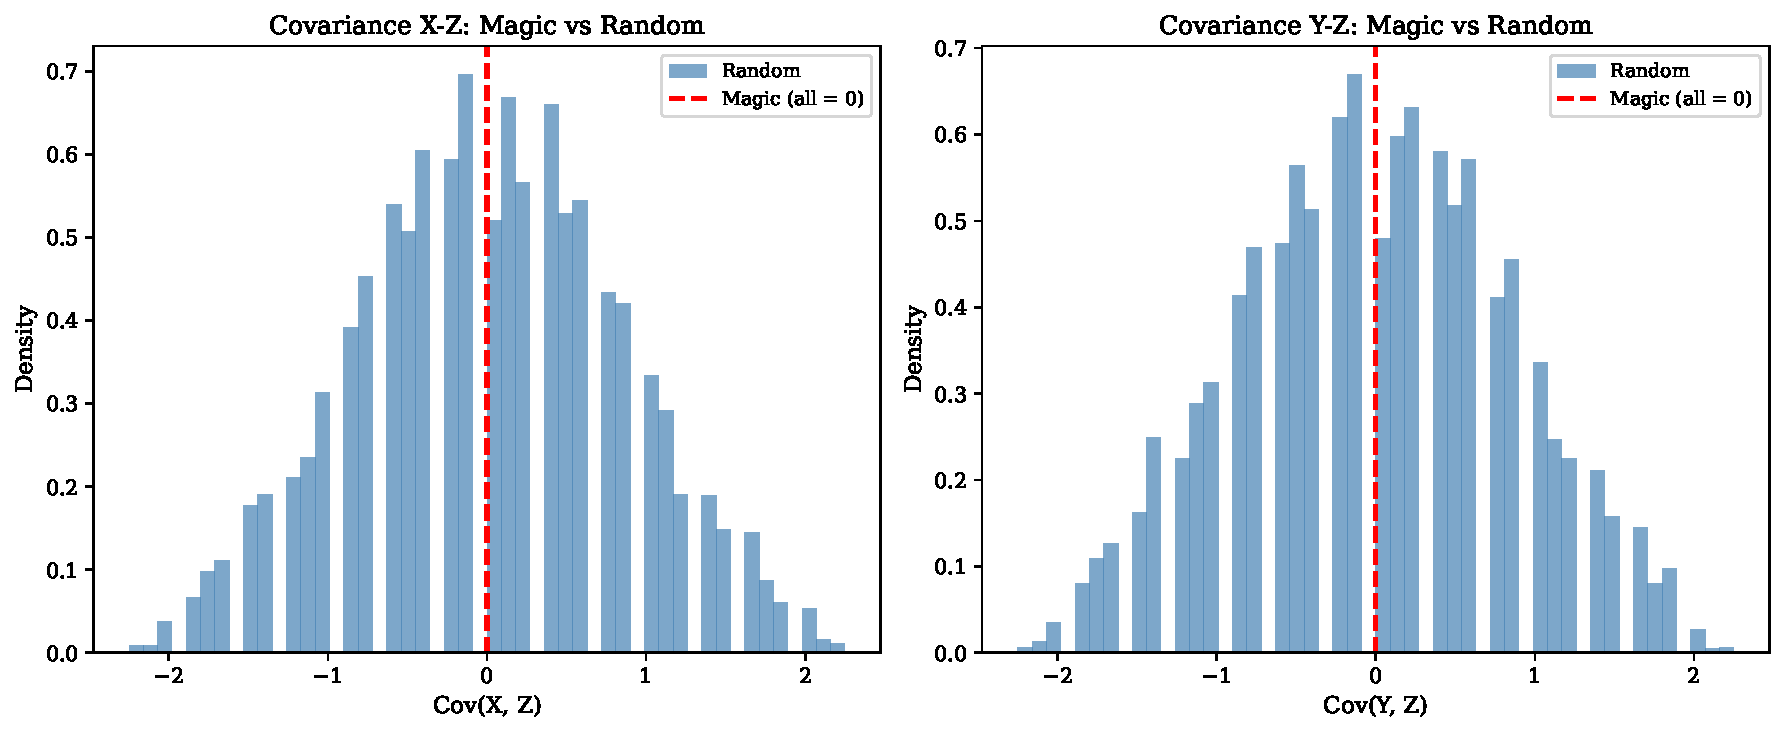
\includegraphics[width=0.9\textwidth]{figures/fig06_covariance_3x3.pdf}
    \caption{Covariance distributions for 5,000 random $3 \times 3$ arrangements.
    The magic square value of exactly zero (red dashed line) lies at the center
    but is achieved by only 8 of 362,880 possible arrangements.}
    \label{fig:covariance_3x3}
\end{figure}

\subsubsection{Geometric Structure}

The $3 \times 3$ Magic Gem comprises nine points, of which eight lie on the convex hull
while the ninth---corresponding to the center cell with value 5---occupies the interior at the origin.
\Cref{fig:magic_gem_3x3} visualizes this structure, with the hull rendered as translucent faces
and vertices colored by their $z$-values.

\begin{figure}[H]
    \centering
    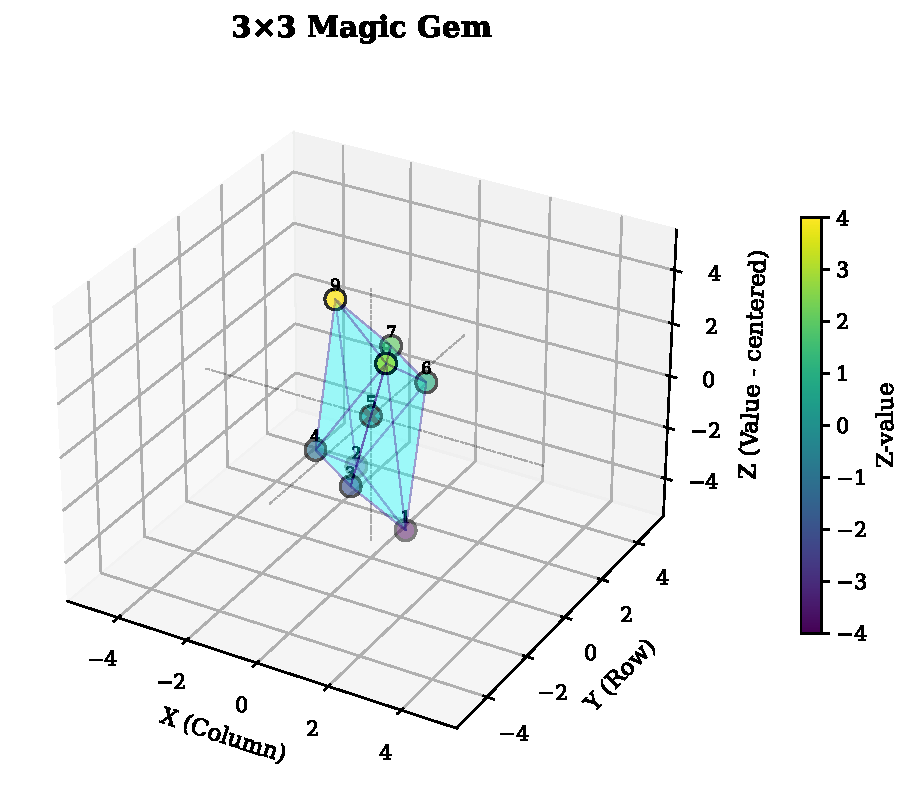
\includegraphics[width=0.7\textwidth]{figures/fig03_magic_gem_3x3.pdf}
    \caption{The $3 \times 3$ Magic Gem showing vertex positions colored by $z$-value
    and the convex hull with translucent faces.
    The center point lies at the origin, interior to the hull.}
    \label{fig:magic_gem_3x3}
\end{figure}

The vector representation, shown in \Cref{fig:vectors_3x3}, displays all nine vectors from the centroid.
The balanced distribution---vectors in each direction having $z$-components 
that sum to zero when weighted by position---visually manifests the zero-covariance property.

\begin{figure}[H]
    \centering
    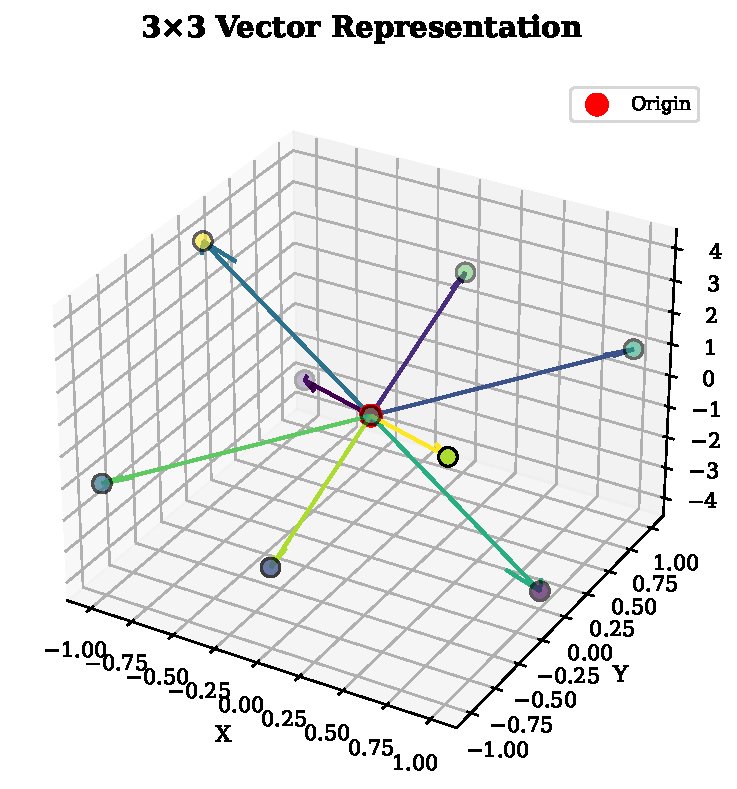
\includegraphics[width=0.7\textwidth]{figures/fig04_vectors_3x3.pdf}
    \caption{Vector representation of the $3 \times 3$ Magic Gem,
    showing nine vectors from the centroid to each vertex.}
    \label{fig:vectors_3x3}
\end{figure}

The hull volume distribution (\Cref{fig:hull_volume_3x3}) places the Magic Gem's volume 
of 18 cubic units near the center of the distribution for random arrangements,
indicating that magic squares are distinguished by their covariance structure
rather than geometric extremality.

\begin{figure}[H]
    \centering
    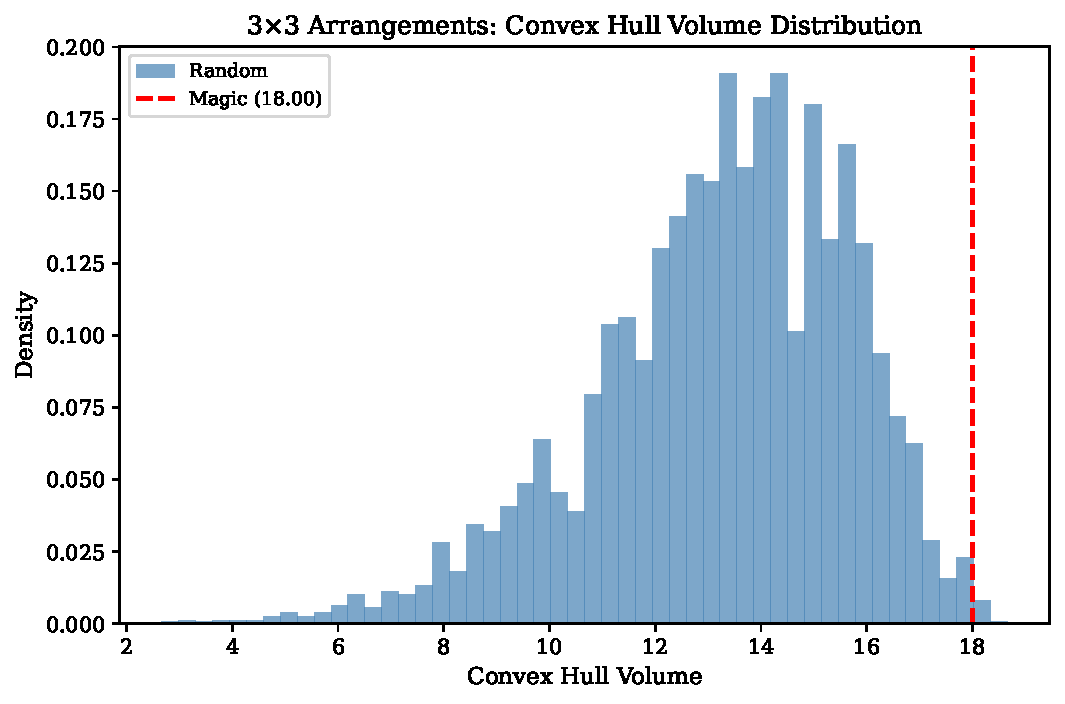
\includegraphics[width=0.7\textwidth]{figures/fig07_hull_volume_3x3.pdf}
    \caption{Convex hull volume distribution for 5,000 random $3 \times 3$ arrangements.
    The Magic Gem volume (red line) lies near the distribution center.}
    \label{fig:hull_volume_3x3}
\end{figure}

\subsection{The 4×4 Case: Even-Order Analysis}

The transition to $n = 4$ introduces several important changes.
First, $4 \times 4$ magic squares require different construction methods than odd orders---the 
doubly-even method replaces the Siamese method.
Second, there exist 880 essentially different $4 \times 4$ magic squares,
providing a richer landscape for geometric study.
Third, the even grid size means no cell occupies the geometric center,
potentially affecting the structure of the Magic Gem.

\subsubsection{Construction and Visualization}

\Cref{fig:magic_square_4x4} shows the $4 \times 4$ magic square constructed via the doubly-even method,
with magic constant $M(4) = 34$.
The construction process, illustrated in \Cref{fig:construction_4x4}, 
follows the same four steps as for odd orders:
grid centering, $z$-value assignment, centering of $z$-values, and hull computation.

\begin{figure}[H]
    \centering
    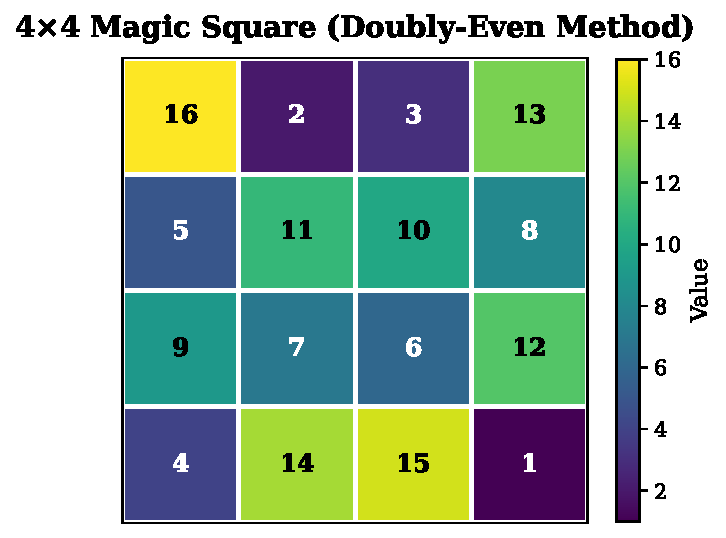
\includegraphics[width=0.45\textwidth]{figures/fig08_magic_square_4x4.pdf}
    \caption{A $4 \times 4$ magic square constructed via the doubly-even method.
    Each row, column, and diagonal sums to $M(4) = 34$.}
    \label{fig:magic_square_4x4}
\end{figure}

\begin{figure}[H]
    \centering
    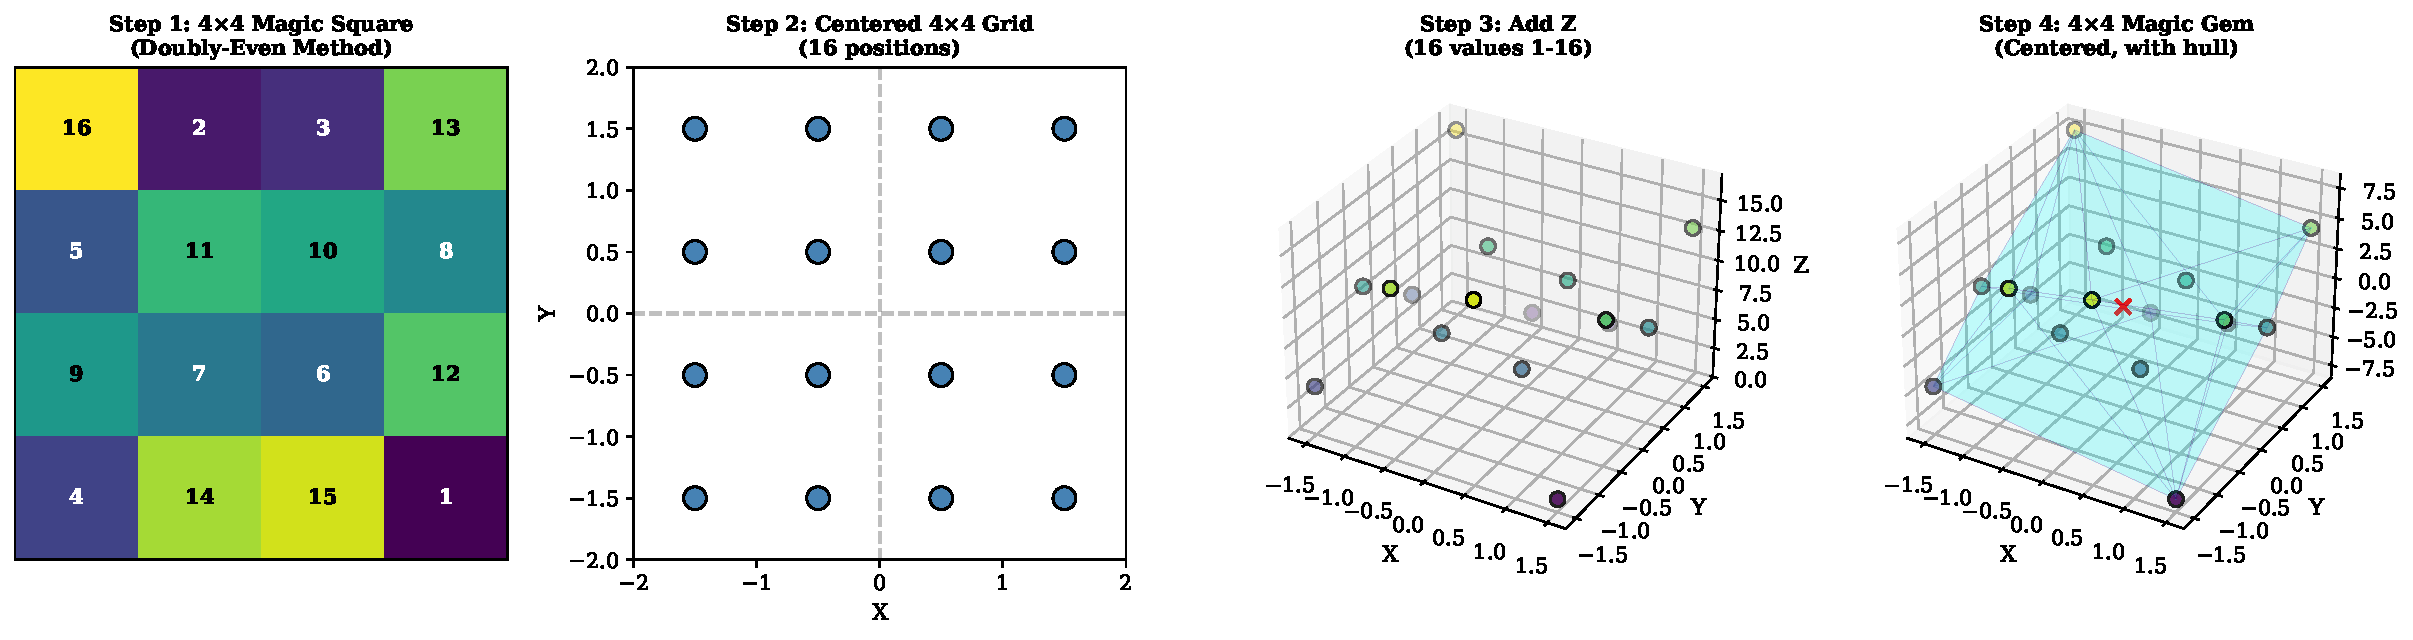
\includegraphics[width=\textwidth]{figures/fig09_construction_4x4.pdf}
    \caption{Construction of the $4 \times 4$ Magic Gem, showing the four-step process
    from magic square to centered polyhedral representation.}
    \label{fig:construction_4x4}
\end{figure}

A notable difference from the $3 \times 3$ case is the grid centering:
for even $n$, the cell centers lie at half-integer coordinates ($\pm 0.5, \pm 1.5$),
and no cell coincides with the origin.
Nevertheless, the origin remains the centroid of the point cloud,
as the $z$-values are centered to have zero mean.

\subsubsection{Zero-Covariance for Even Order}

The Zero-Covariance Theorem makes no distinction between even and odd orders,
predicting $\Cov(X, Z) = \Cov(Y, Z) = 0$ for all magic squares.
Our computations confirm this prediction for the $4 \times 4$ case:
the magic square achieves exactly zero covariance to machine precision.

\Cref{fig:covariance_4x4} compares the magic covariance to 3,000 random $4 \times 4$ arrangements.
The distributions are somewhat narrower than for $3 \times 3$ (relative to their range),
reflecting the increased constraints imposed by having 16 cells rather than 9.
The magic square again sits precisely at zero.

\begin{figure}[H]
    \centering
    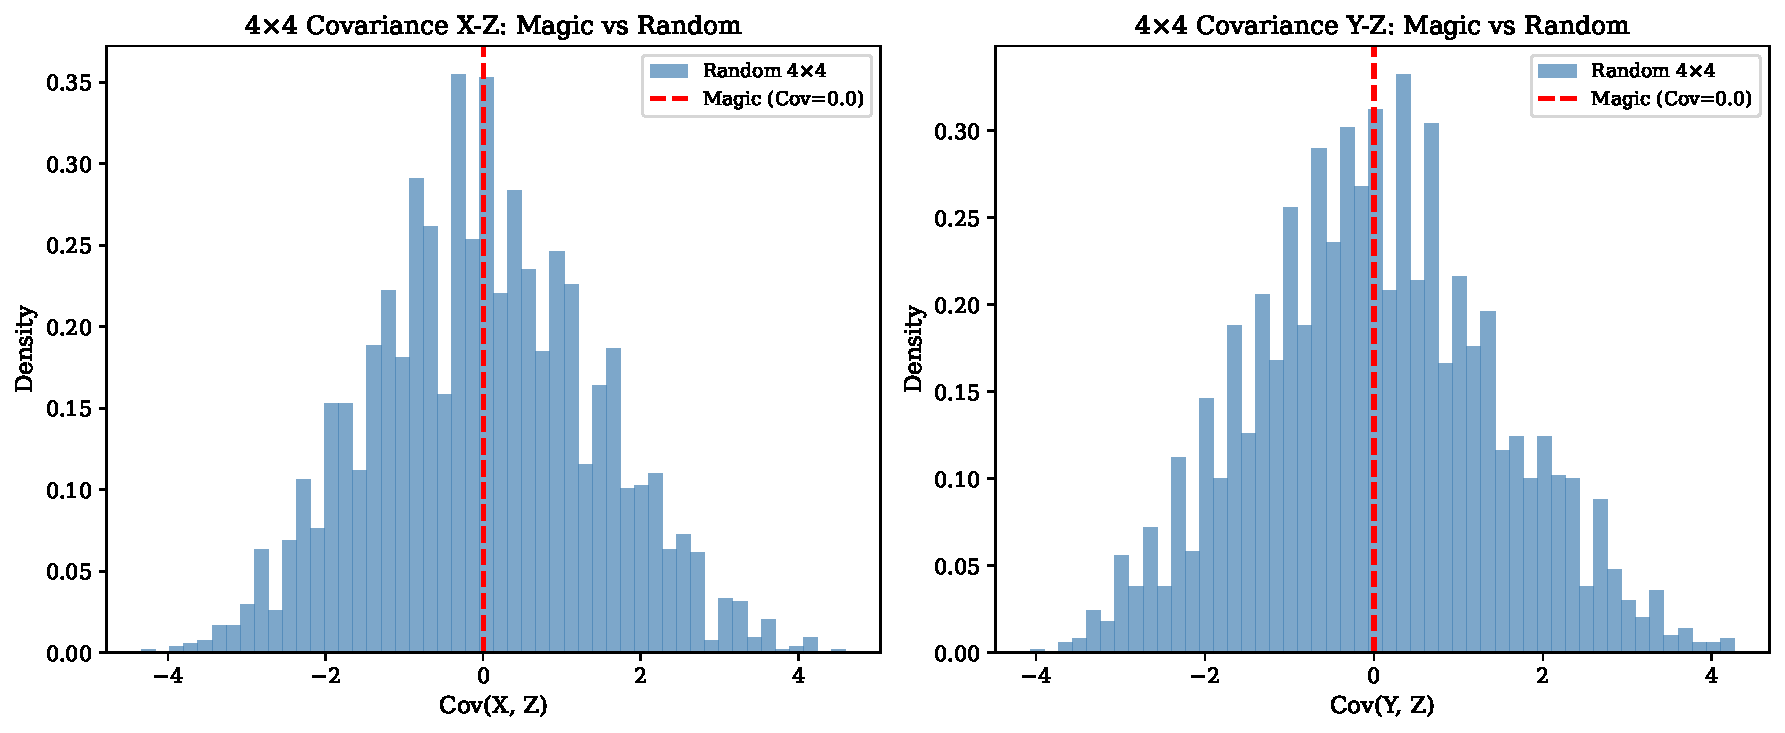
\includegraphics[width=0.9\textwidth]{figures/fig12_covariance_4x4.pdf}
    \caption{Covariance distributions for 3,000 random $4 \times 4$ arrangements,
    with the magic square value of exactly zero marked.}
    \label{fig:covariance_4x4}
\end{figure}

\subsubsection{Geometric Properties}

The $4 \times 4$ Magic Gem, shown in \Cref{fig:magic_gem_4x4}, has 16 vertices.
Unlike the $3 \times 3$ case where only one point (the center) is interior,
the $4 \times 4$ gem has multiple interior points, with approximately 12 vertices on the hull.

\begin{figure}[H]
    \centering
    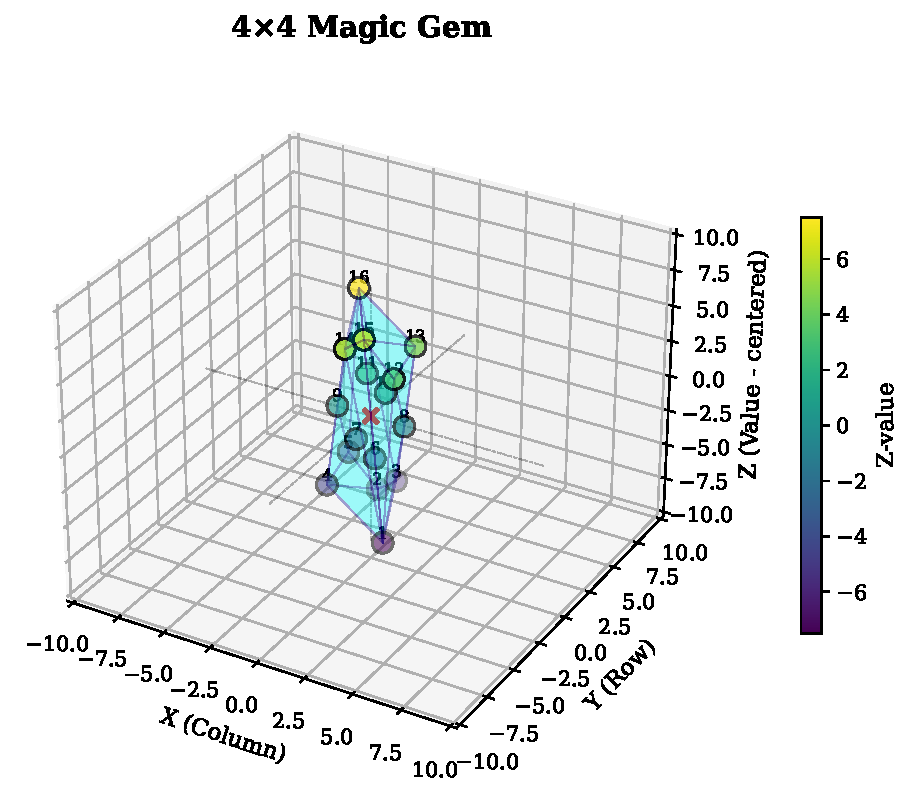
\includegraphics[width=0.7\textwidth]{figures/fig10_magic_gem_4x4.pdf}
    \caption{The $4 \times 4$ Magic Gem showing 16 vertices colored by $z$-value.
    The more complex structure reflects the larger grid size.}
    \label{fig:magic_gem_4x4}
\end{figure}

The vector representation (\Cref{fig:vectors_4x4}) displays 16 vectors from the centroid.
Despite the absence of a central cell, the vectors remain balanced according to the zero-covariance criterion.

\begin{figure}[H]
    \centering
    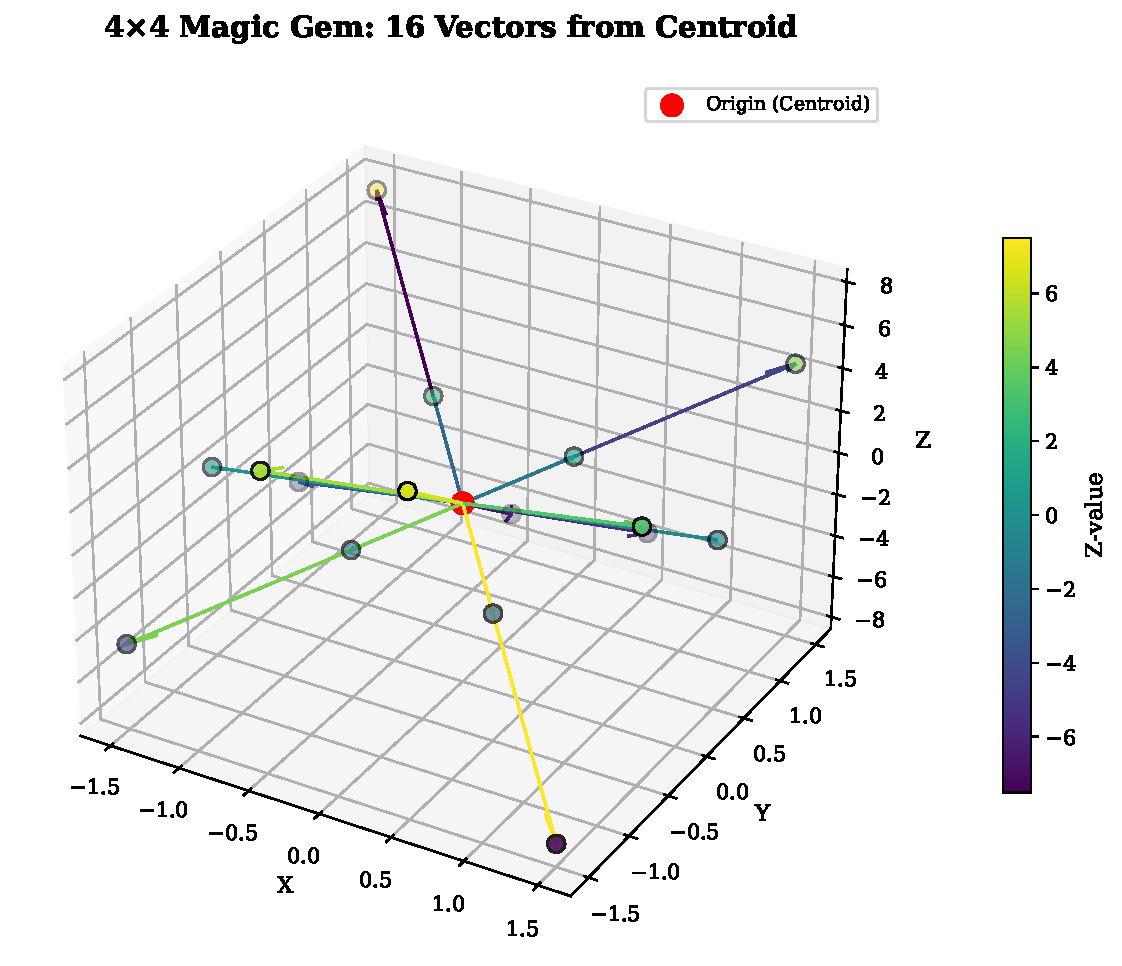
\includegraphics[width=0.7\textwidth]{figures/fig11_vectors_4x4.pdf}
    \caption{Vector representation of the $4 \times 4$ Magic Gem,
    showing 16 vectors from the centroid.}
    \label{fig:vectors_4x4}
\end{figure}

\Cref{fig:hull_volume_4x4} shows the hull volume distribution for random $4 \times 4$ arrangements.
As with the $3 \times 3$ case, the Magic Gem volume falls near the center of the distribution.

\begin{figure}[H]
    \centering
    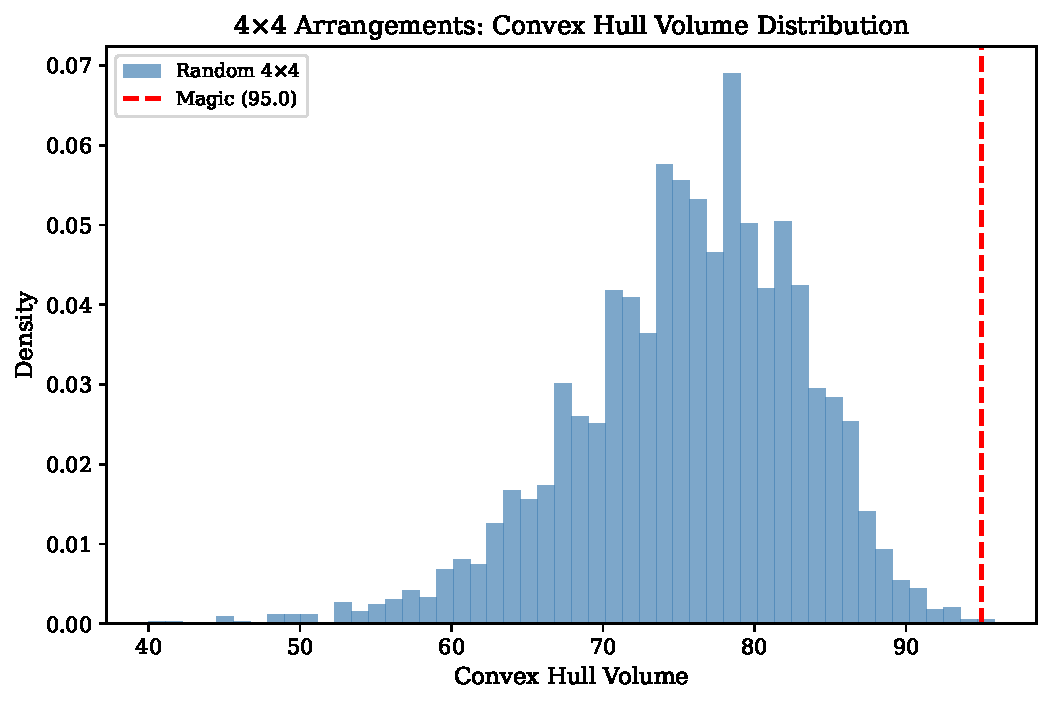
\includegraphics[width=0.7\textwidth]{figures/fig13_hull_volume_4x4.pdf}
    \caption{Convex hull volume distribution for 3,000 random $4 \times 4$ arrangements.}
    \label{fig:hull_volume_4x4}
\end{figure}

\subsection{The 5×5 Case: Return to Odd Order}

Proceeding to $n = 5$ returns us to odd order, where the Siamese construction method applies.
The $5 \times 5$ case is substantially more complex:
there exist approximately 275 million magic squares forming about 34 million equivalence classes.

\subsubsection{Construction and Visualization}

\Cref{fig:magic_square_5x5} shows the $5 \times 5$ magic square with magic constant $M(5) = 65$.
The Siamese method produces a characteristic diagonal pattern visible in the arrangement.

\begin{figure}[H]
    \centering
    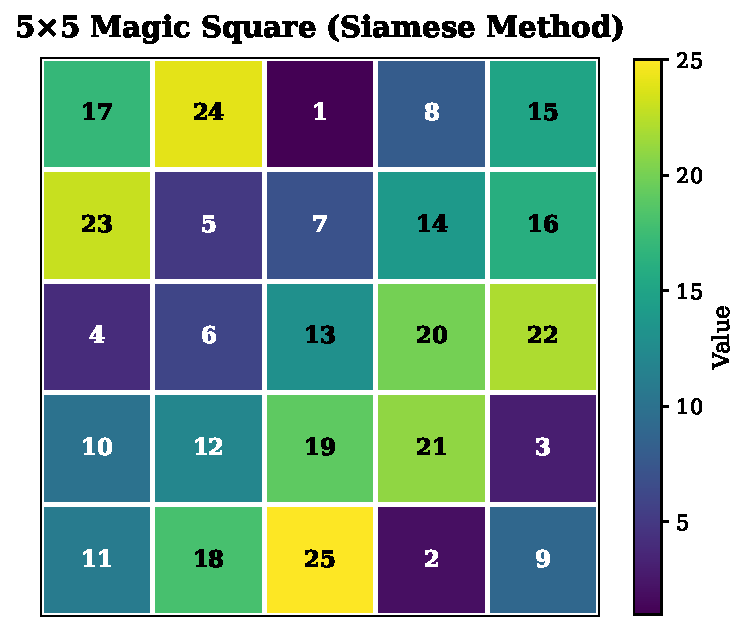
\includegraphics[width=0.5\textwidth]{figures/fig14_magic_square_5x5.pdf}
    \caption{A $5 \times 5$ magic square constructed via the Siamese method.
    Each row, column, and diagonal sums to $M(5) = 65$.}
    \label{fig:magic_square_5x5}
\end{figure}

The construction process (\Cref{fig:construction_5x5}) maps the 25-cell grid 
to 25 points in $\R^3$, with the central cell again coinciding with the origin.

\begin{figure}[H]
    \centering
    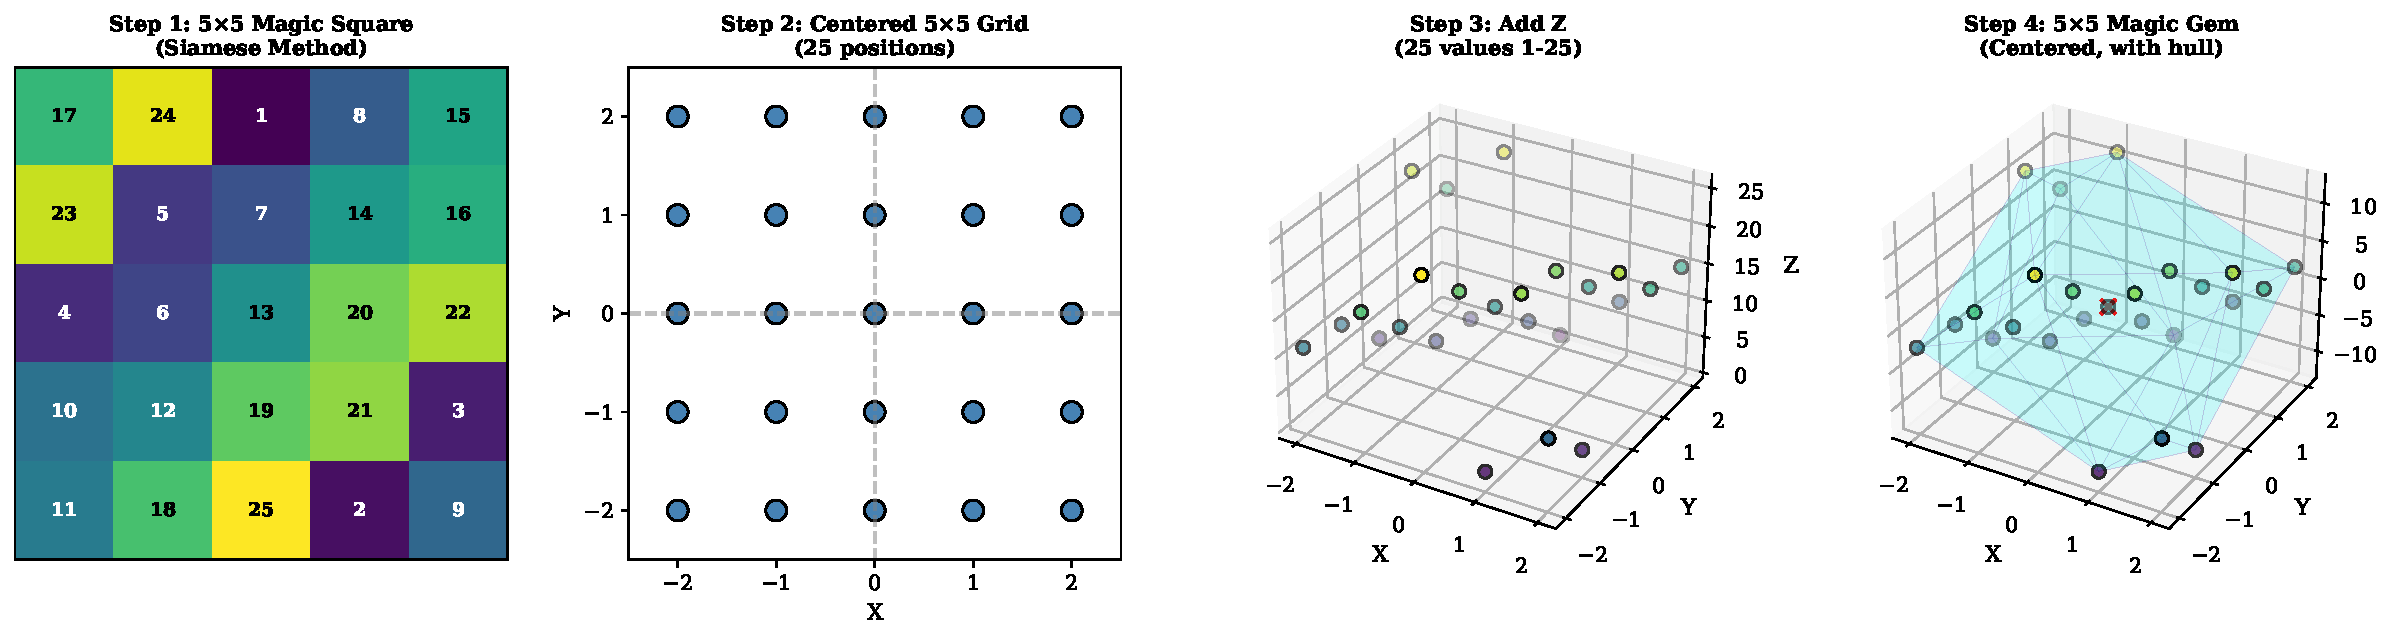
\includegraphics[width=\textwidth]{figures/fig15_construction_5x5.pdf}
    \caption{Construction of the $5 \times 5$ Magic Gem.}
    \label{fig:construction_5x5}
\end{figure}

\subsubsection{Zero-Covariance Verification}

The $5 \times 5$ magic square achieves $\Cov(X, Z) = \Cov(Y, Z) = 0$ exactly,
as predicted by the theorem.
\Cref{fig:covariance_5x5} compares this to 3,000 random arrangements.
The covariance distributions are wider than for smaller orders
(reflecting the larger range of values 1--25),
but the magic square remains precisely at zero.

\begin{figure}[H]
    \centering
    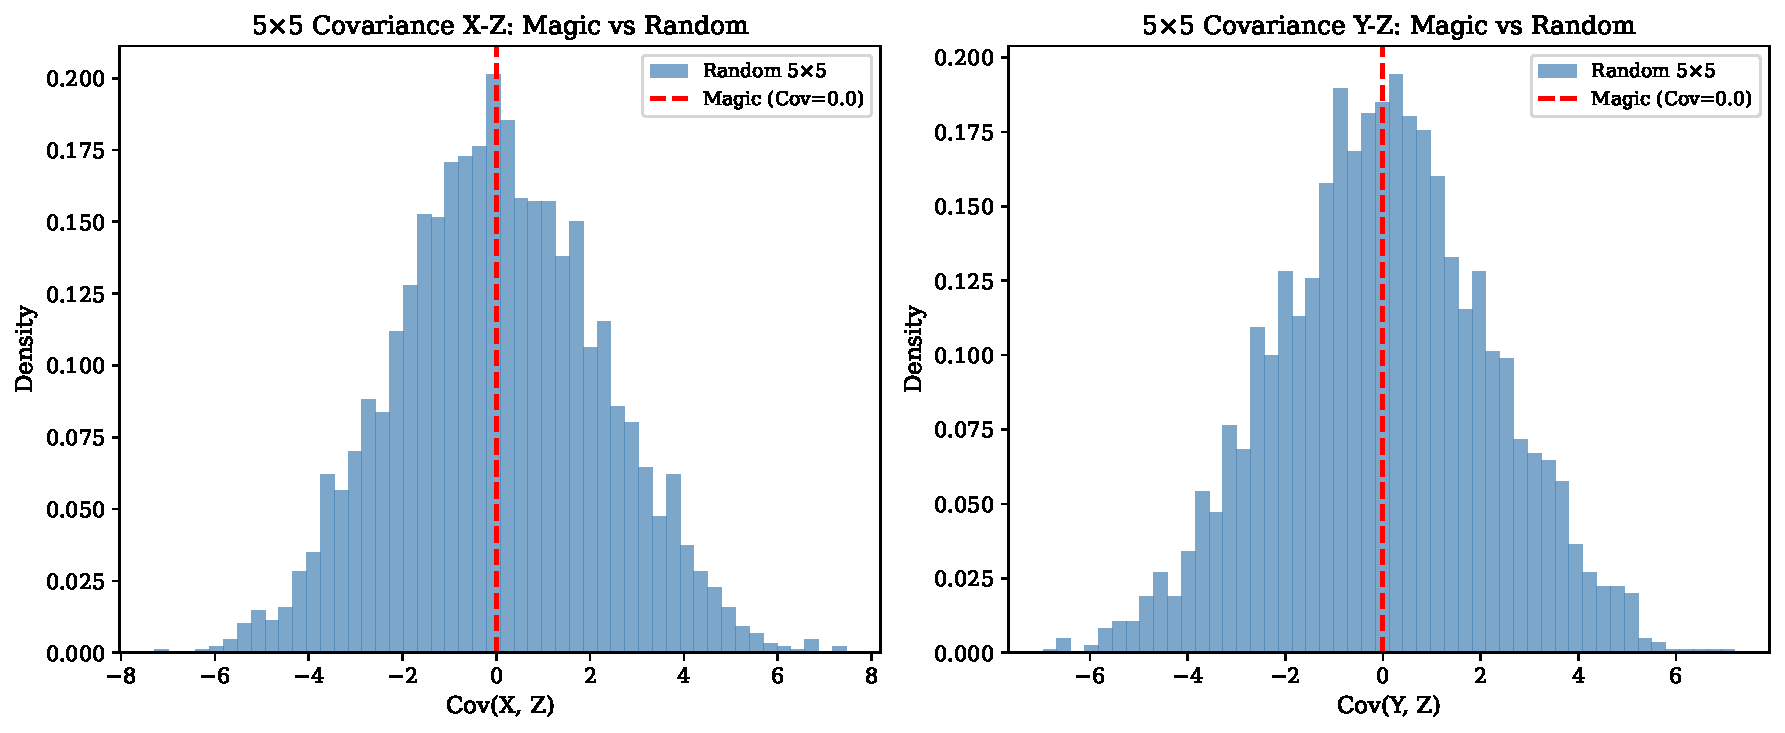
\includegraphics[width=0.9\textwidth]{figures/fig18_covariance_5x5.pdf}
    \caption{Covariance distributions for 3,000 random $5 \times 5$ arrangements.
    The wider spread reflects the larger value range, but magic squares still achieve exactly zero.}
    \label{fig:covariance_5x5}
\end{figure}

\subsubsection{Geometric Properties}

The $5 \times 5$ Magic Gem (\Cref{fig:magic_gem_5x5}) exhibits substantially greater complexity.
Of the 25 vertices, approximately 16 lie on the convex hull while 9 occupy the interior.
The vector representation (\Cref{fig:vectors_5x5}) shows the balanced distribution of 25 vectors.

\begin{figure}[H]
    \centering
    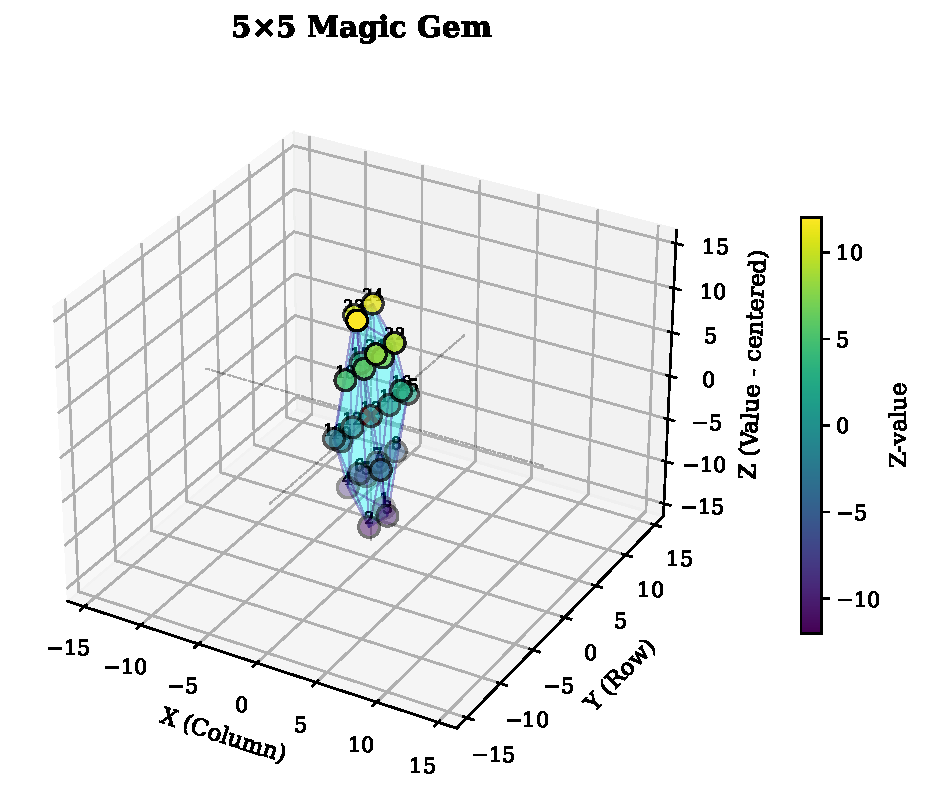
\includegraphics[width=0.7\textwidth]{figures/fig16_magic_gem_5x5.pdf}
    \caption{The $5 \times 5$ Magic Gem showing 25 vertices and the convex hull.}
    \label{fig:magic_gem_5x5}
\end{figure}

\begin{figure}[H]
    \centering
    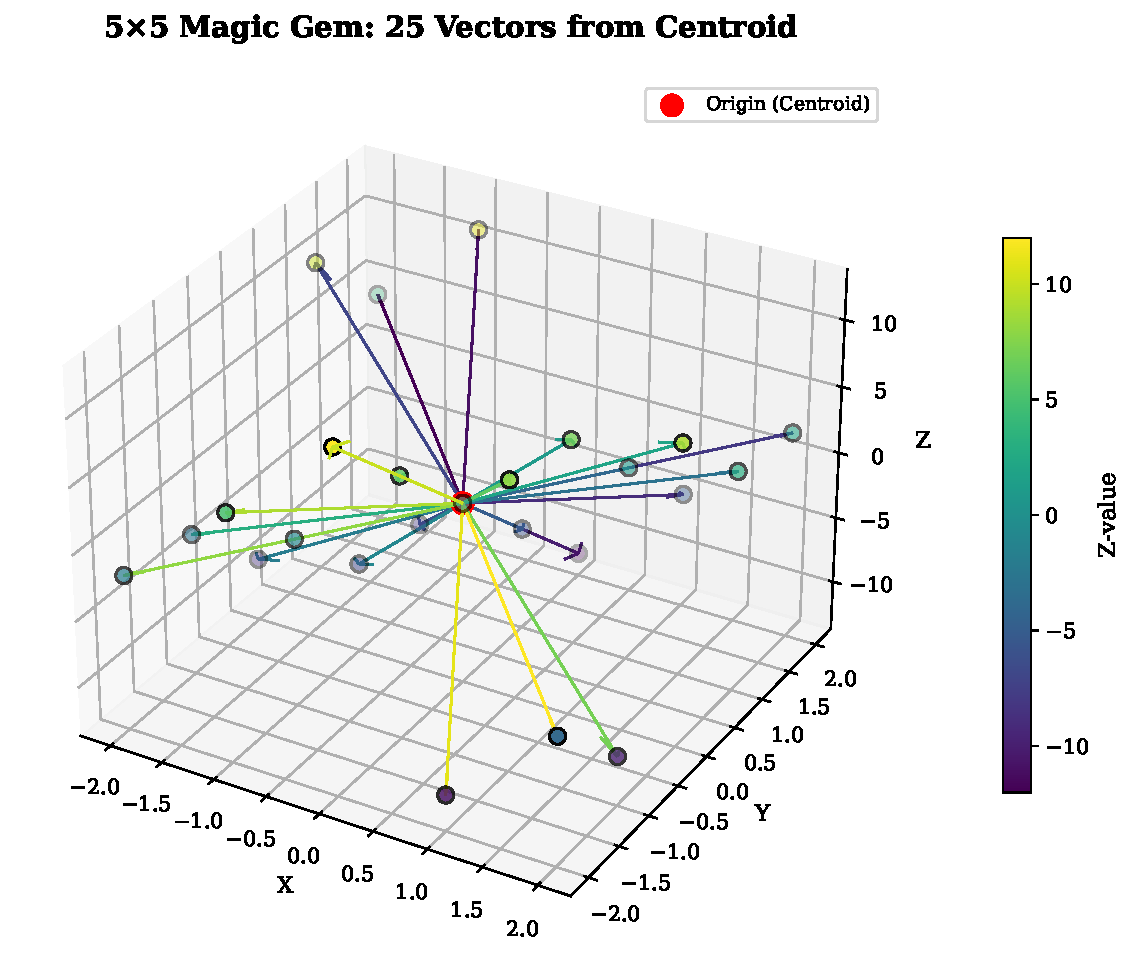
\includegraphics[width=0.7\textwidth]{figures/fig17_vectors_5x5.pdf}
    \caption{Vector representation of the $5 \times 5$ Magic Gem.}
    \label{fig:vectors_5x5}
\end{figure}

\begin{figure}[H]
    \centering
    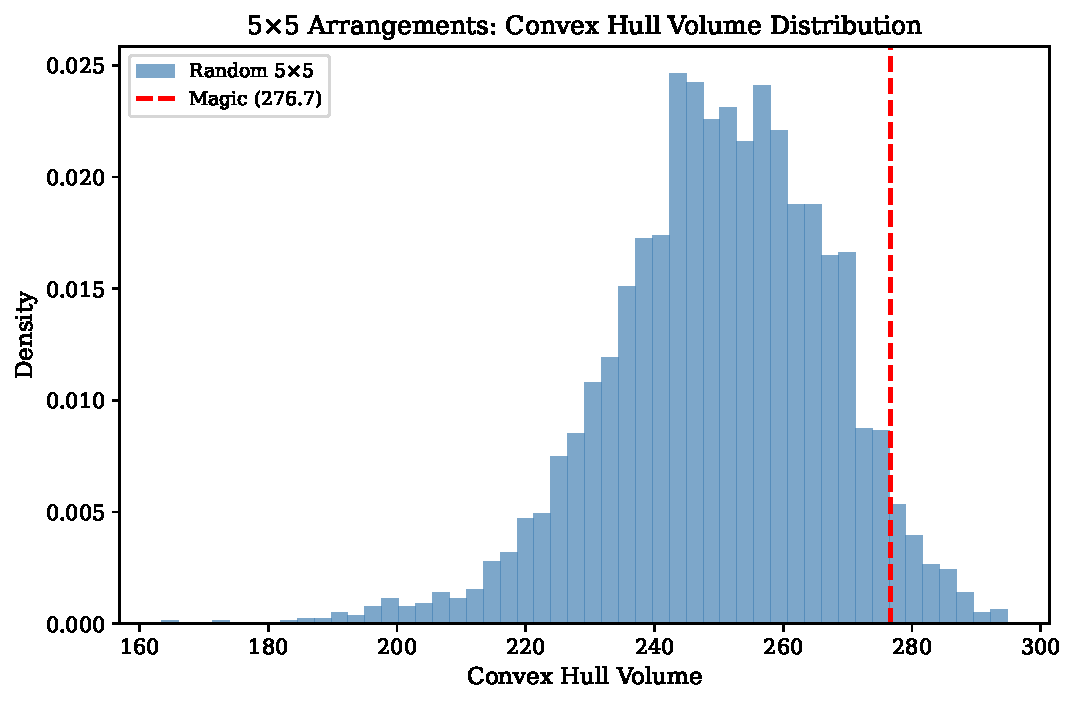
\includegraphics[width=0.7\textwidth]{figures/fig19_hull_volume_5x5.pdf}
    \caption{Convex hull volume distribution for 3,000 random $5 \times 5$ arrangements.}
    \label{fig:hull_volume_5x5}
\end{figure}

\subsection{Cross-Order Comparison}

\Cref{fig:comparison_all} provides a unified view of Magic Gems across all three orders,
highlighting the progression in complexity while maintaining the invariant zero-covariance property.

\begin{figure}[H]
    \centering
    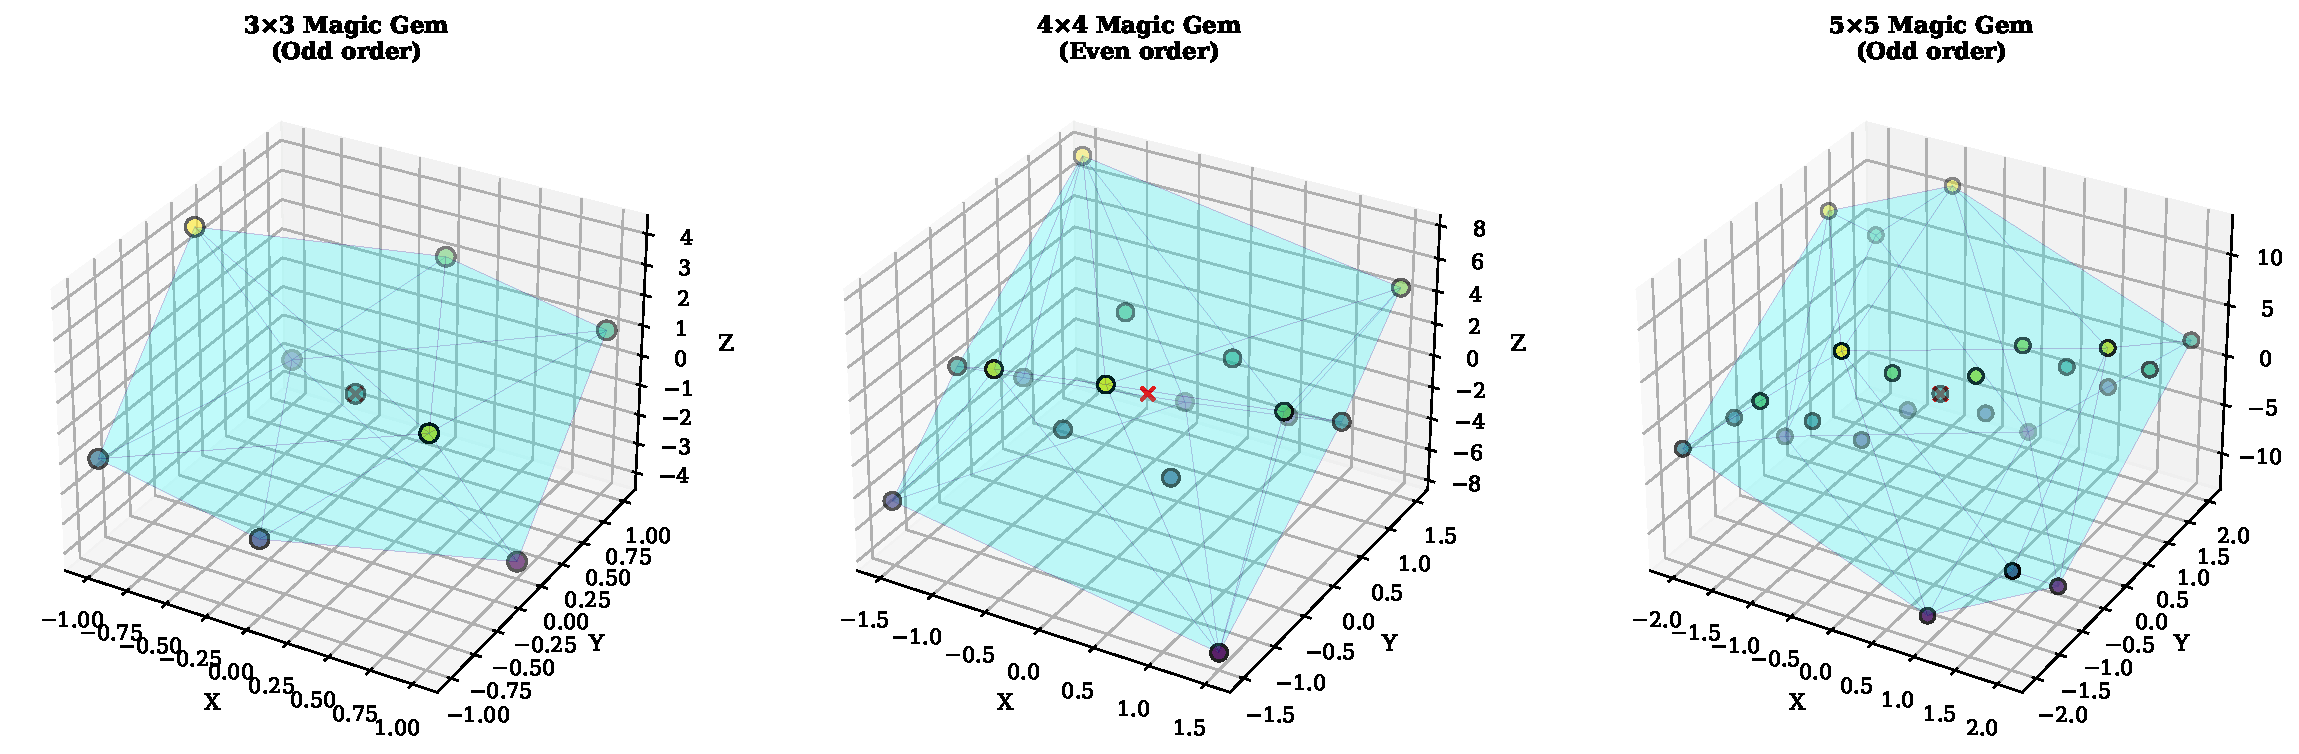
\includegraphics[width=\textwidth]{figures/fig20_comparison_all_orders.pdf}
    \caption{Side-by-side comparison of $3 \times 3$, $4 \times 4$, and $5 \times 5$ Magic Gems.
    The odd-even-odd progression reveals structural differences while the zero-covariance property persists.}
    \label{fig:comparison_all}
\end{figure}

\Cref{tab:comparison_all} summarizes key properties across orders,
demonstrating both the growth in complexity and the invariance of the zero-covariance characterization.

\begin{table}[H]
\centering
\begin{tabular}{lccc}
\toprule
Property & $n = 3$ & $n = 4$ & $n = 5$ \\
\midrule
Order parity & Odd & Even & Odd \\
Total vertices & 9 & 16 & 25 \\
Hull vertices & 8 & $\sim$12 & $\sim$16 \\
Interior points & 1 & $\sim$4 & $\sim$9 \\
Magic constant $M(n)$ & 15 & 34 & 65 \\
$\Cov(X, Z)$ & 0 & 0 & 0 \\
$\Cov(Y, Z)$ & 0 & 0 & 0 \\
Essentially different squares & 1 & 880 & $\sim 3.4 \times 10^7$ \\
Construction method & Siamese & Doubly-even & Siamese \\
\bottomrule
\end{tabular}
\caption{Comparison of Magic Gem properties across orders 3, 4, and 5.
Despite differences in parity, construction method, and complexity,
all orders satisfy the zero-covariance theorem.}
\label{tab:comparison_all}
\end{table}

The even-order case ($n = 4$) demonstrates that the zero-covariance property
does not depend on having a central cell at the origin.
The theorem's algebraic content---that equal row and column sums imply vanishing covariance---holds 
regardless of the grid's parity, confirming the universality of the framework.
